\documentclass{article}
\usepackage[utf8]{inputenc}
\usepackage{graphicx}
\usepackage{amsmath}
\usepackage{hyperref}
\usepackage{stackengine,amssymb,graphicx}
\newcommand\DDiamond{\ensurestackMath{%
  \stackengine{.5pt}{\Diamond}{\scalebox{.75}[1]{$-$}}{O}{c}{F}{F}{L}}}

\newcommand{\sol}{\textbf{solution}}

\title{CSE105/209A: Modern Algorithmic Toolbox\footnote{PI: Vaggos Chatziafratis}, PSET-1\\ }
\author{}
\date{}
\begin{document}
\maketitle
\vspace{-2cm}
\paragraph{Instructions:} Deadline in \textbf{7 days from day of posting, 11:59pm}. Prepare a pdf of your solutions, with your name and ucsc id number. Feel free to discuss solutions with your colleagues (other students), explore the internet, read and be inspired from the textbooks etc. But what you type should be typed by you and you only in latex. In algorithms, we appreciate brevity and accuracy: your solutions should be to the point, often one or two sentences suffice to provide all necessary details and descriptions. Unnecessarily long answers will not get full credit. You will submit your pdf either on canvas or gradescope, more details to follow.\\











\noindent \textbf{Ex.1 (20pts) (Graphs and Matrices)}

Throughout this exercise we think of the adjacency representation of an undirected graph $G$ with $n$ vertices and $m$ edges. Each entry $A[i,j]$ in the adjacency matrix $A$ is $1$ \textbf{if and only if} the edge $(i,j)$ is present (if the edge $(i,j)$ is not present, let's say the entry is 0). All diagonal entries in $A$ are 0 since there are no self-loops.

\begin{enumerate}
    \item For a cycle on $5$ nodes, write down explicitly its adjacency matrix. Compute and write down $A^2,A^3$. 
    
    \begin{equation}
        A = \begin{pmatrix}
            0 & 1 & 0 & 0 & 1 \\
            1 & 0 & 1 & 0 & 0 \\
            0 & 1 & 0 & 1 & 0 \\
            0 & 0 & 1 & 0 & 1 \\
            1 & 0 & 0 & 1 & 0
        \end{pmatrix}
    \end{equation}

    $$A^2 = \begin{pmatrix}
2 & 0 & 1 & 1 & 0 \\
0 & 2 & 0 & 1 & 1 \\
1 & 0 & 2 & 0 & 1 \\
1 & 1 & 0 & 2 & 0 \\
0 & 1 & 1 & 0 & 2
\end{pmatrix}$$

$$A^3 = \begin{pmatrix}
0 & 3 & 1 & 1 & 3 \\
3 & 0 & 3 & 1 & 1 \\
1 & 3 & 0 & 3 & 1 \\
1 & 1 & 3 & 0 & 3 \\
3 & 1 & 1 & 3 & 0
\end{pmatrix}$$

    \item For a path on $5$ nodes, write down explicitly its adjacency matrix. Compute and write down $A^2,A^3$.
    
    $$A = \begin{pmatrix} 0 & 1 & 0 & 0 & 0 \\ 1 & 0 & 1 & 0 & 0 \\ 0 & 1 & 0 & 1 & 0 \\ 0 & 0 & 1 & 0 & 1 \\ 0 & 0 & 0 & 1 & 0 \end{pmatrix}$$

    $$A^2 = \begin{pmatrix} 1 & 0 & 1 & 0 & 0 \\ 0 & 2 & 0 & 1 & 0 \\ 1 & 0 & 2 & 0 & 1 \\ 0 & 1 & 0 & 2 & 0 \\ 0 & 0 & 1 & 0 & 1 \end{pmatrix}$$

    $$A^3  = \begin{pmatrix} 0 & 2 & 0 & 1 & 0 \\ 2 & 0 & 3 & 0 & 1 \\ 0 & 3 & 0 & 3 & 0 \\ 1 & 0 & 3 & 0 & 2 \\ 0 & 1 & 0 & 2 & 0 \end{pmatrix}$$

    \item Generally, suppose you are given a cycle on $n$ nodes. Start from $A$ and keep multiplying it with itself until you get matrix $B=A^k$ for some integer number $k$. What is the smallest value of $k$ such that all of $B$'s non-diagonal entries are non-zero? (Hint: maybe different answer for odd or even $n$.)
    
    \textbf{solution}

    If the cycle has an even number of nodes, the nondiagonals will never become all nonzero. every node cycles between being reachable and not reachable in the cycle. 

    if a cycle has an odd number of nodes, the nondiagonals will take \(n-1\) steps to be all nonzero. It takes at least \(n-1\) steps to ensure the direct neighbors of the starting vertex are always occupied at least once on all subsequent walk lengths. 

    


    \item Generally, suppose you are given a path on $n$ nodes. Start from $A$ and keep multiplying it with itself until you get matrix $C=A^k$ for some integer number $k$. What is the smallest value of $k$ such that all of $B$'s non-diagonal entries are non-zero? (Hint: maybe different answer for odd or even $n$, or maybe not...)
    
    \textbf{solution}

    Note a path is bipartite. Every step goes from right to left, or left to right, thus it is impossible for one to reach every node on even or odd step lengths. 



    \item \textbf{BONUS:} How would your answers above change if the graphs were directed instead?
    

    \textbf{solution}

    the solutions that are false remain false. the odd numbered cycle also becomes false since there is only one path at every step. 
\end{enumerate}

\newpage
For this exercise, we don't require a formal proof, but we want to see some sufficiently justified explanation for your responses based on what we discussed in class.\\


\noindent \textbf{Ex.2 (20pts) (BFS, but slower)}

Imagine you you are given a graph $G$ with adjacency matrix $A$, but you forgot how to implement the BFS algorithm. But luckily you have access to MatMul, a programming language that only allows you to do matrix multiplications, and check any entry that you want from $A$ or the subsequent multiplications with itself.

\begin{enumerate}
    \item How would you check whether there is a node of degree 2023 in the graph?
    
    \sol

    square the adjacency matrix, then check along the diagonal if there is a value of 2023. Paths of length two that reach back to the original node are in direct correspondance with the degree of the vertex. 

    \item How would you count the triangles in the graph?
    
    \sol

    as discussed in class, cubing the matrix, summing the trace then dividing by 6 results in the trangle count. the diagonal along the matrix after cubing the matrix gives the paths of length 3 back to the original node, which is a triangle. these triangles are sextuple counted since each triangle has 3 vertecies, and the paths can go in two directions. 

    \item How would you check whether or not the graph is connected?
    
    \sol 

    we can calculate the second eigenvalue of the laplacian matrix. the laplacian matrix is formed by squaring the original matrix, then taking only the diagonal and subtracting the original matrix from it. Then we take the characteristic polynomial to find the eigenvalues. if the second smallest eigenvalue is 0, then it is not connected. if it is not zero, then it is connected. This is because if a graph is disconnected, the vertecies can be permuted and can be written as a block diagonal matrix. Since every laplacian matrix has smallest eigenvalue zero, each block diagonal matrix produces an eigenvector of all ones on indecies the block matrix occupies. this is guaranteed to be an eigenvector for each block matrix, and since there are 1 for each disconnected component in the graph, there must be at least 2 0 eigenvalues if the graph is disconnected.

    if the graph is connected, then the second eigenvalue must be nonzero. 

    consider the quadratic form of the laplacian. 

    $$\mathbf{x}^T L \mathbf{x} = \sum_{(u,v) \in E} (x_u - x_v)^2$$

    this sum must be zero if the eigenvalue of x is zero, since \(Lx=0\) on the LHS. every term must then also be zero since the sum is monotone increasing. In a connected graph, since every edge \(u,v\) is connected, every value \(x_i\) must be 1. therefore the only vector that has eigenvalue 0 is the all 1s vector. 



\end{enumerate}

\newpage

\noindent \textbf{Ex.3 (20pts) (Bipartite and Traces)}

Prove that an undirected graph is bipartite if and only if the following holds:
\[
trace(A^{2k+1})=0, \forall k\in \mathbf{N}=\{0,1,2,3,\ldots\}
\]

\sol 

\(trace(A^{2k+1})=0\) is equivalent to saying there are no odd length cycles. also note that two coloring is the same as bipartiteness. if there is an odd length cycle, then that cycle cannot be two colored because of the parity. 

\newpage


\noindent \textbf{Ex.4 (20pts) (Other Motifs)}
See Figure 1 that shows two motif equations that relate properties of the adjacency matrix $A$ (more specifically, entries of its square $A^2$) and hidden patterns in the graph. We ask you to prove these two motif equations. Here the patterns shown at the right-hand-side of the equations are: 

\begin{itemize}
    \item $K_4$: this is the clique on 4 nodes, that is the graph where every edge between two nodes is present.
    \item $\DDiamond$: this is the diamond symbol, that is the graph on 4 nodes, where exactly one edge is missing (as shown, the one connecting the top and bottom vertices.)
    \item $C_4$: this is the cycle on 4 nodes (i.e., a square).
\end{itemize}


\begin{figure}[ht]
    \centering
    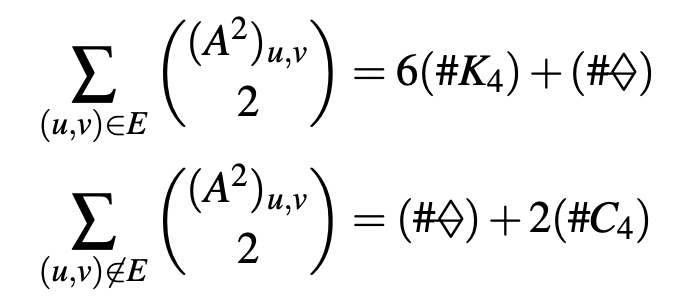
\includegraphics{patterns.png}
    \caption{Two Motif Equations.}
    \label{fig:my_label}
\end{figure}

\sol 

\begin{enumerate}
    \item assume arbitrary two verticies \(u,v\) that are edges. \(A^2\) counts the number of these distance two paths. for each of these, if we choose 2 then this forms a 4 vertex subgraph, however we dont know how the internal edges are, other than \(uv\) is an edge. Since there is an internal edge, it must not count any cycles. diamonds are counted once since for each diamond, the sum checks only the diagonal edge which shows up once. A clique is counted 6 times because cliques on 4 vertecies have 6 edges and each edge contributes once to the count. 


    \item assume arbitrary two verticies \(u,v\) that are not edges. \(A^2\) counts the number of these distance two paths. for each of these, if we choose 2 then this forms a 4 vertex subgraph, however we dont know how the internal edges are, other than \(uv\) is not an edge. since \(uv\) is not an edge, any \(uv\) and choose two other edges must not be a clique. if it is a cycle, then it is double counted (if the 4 vertecies are \(u,v,w,z\), \(uv\) is not an edge and contributes once to the count, then \(wz\) contributes another). if it is a diamond, only the non-edge contributes once to the count. 
\end{enumerate}



\newpage
\noindent \textbf{Ex.5 (20pts) (Strassen's algorithm)}
Devise a divide and conquer algorithm that multiplies a matrix $A$ and a matrix $B$ (both of them are $n$-by-$n$) in time $O(n^{\log_2 7})$. This improves over the naive $O(n^3)$ algorithm we learned in high-school.

Your answer should be a clear exposition of the steps needed to perform the multiplication, and also a proof for its runtime. If it helps feel free to assume that $n$ is a power of $2$.

\sol 

Assume that the matrix is of shape \(2^n\) by \(2^n\). If the matrix is not this shape, pad out the matrix with zeros until it is of this size. asymptotically this does not affect runtime. 

Divide the matrix into four quadrants. There exists a way to mix and match different sums of the four quadrants and multiply them together such that direct combinations of sums and differences result in the final matrix result we wished to attain. 

First note, matrix multiplication distributes over addition. Given 
\begin{equation}
    A = \begin{pmatrix} a & b \\ c & d \end{pmatrix}, 
    B = \begin{pmatrix} e & f \\ g & h \end{pmatrix}
\end{equation}

the naive algorithm uses 8 multiplications to achieve the desired C matrix 


\begin{equation}
    \begin{split}
        C_{1,1} &= ae + bg\\
        C_{1,2} &= af + bh\\
        C_{2,1} &= ce + dg\\
        C_{2,2} &= cf + dh\\
    \end{split}
\end{equation}


but strassen uses different values to calculate each \(C_{i,j}\), namely

\begin{equation}
    \begin{split}
        P_1 &= A_{1,1}(B_{1,2} - B_{2,2})\\
        P_2 &= (A_{1,1} + A_{1,2})B_{2,2}\\
        P_3 &= (A_{2,1} + A_{2,2})B_{1,1}\\
        P_4 &= A_{2,2}(B_{2,1} - B_{1,1})\\
        P_5& = (A_{1,1} + A_{2,2})(B_{1,1} + B_{2,2})\\
        P_6& = (A_{1,2} - A_{2,2})(B_{2,1} + B_{2,2})\\
        P_7 &= (A_{1,1} - A_{2,1})(B_{1,1} + B_{1,2})
    \end{split}
\end{equation}

and 

\begin{equation}
    \begin{split}
        C_{1,1} &= P_5 + P_4 - P_2 + P_6\\
        C_{1,2} &= P_1 + P_2\\
        C_{2,1} &= P_3 + P_4\\
        C_{2,2} &= P_1 + P_5 - P_3 - P_7
    \end{split}
\end{equation}


\end{document}

